\documentclass[14pt]{extreport}
\usepackage{cmap}
\usepackage[utf8]{inputenc}
\usepackage[english,ukrainian]{babel}
\usepackage{graphicx}
\usepackage{geometry}
\usepackage{listings}
\usepackage{amsmath}
\usepackage{float}
\geometry{
	a4paper,
	left=20mm,
	right=20mm,
	top=20mm,
	bottom=20mm
}
\lstset{
	language=bash,
	tabsize=4,
	breaklines,
	keepspaces,
	showstringspaces=false,
}
\graphicspath{ {./pictures} }
\setlength{\parindent}{4em}

\newcommand\subject{Конструювання програмного забезпечення}
\newcommand\lecturer{доцент кафедри ПЗ\\Сердюк П.В.}
\newcommand\teacher{доцент кафедри ПЗ\\Сердюк П.В.}
\newcommand\mygroup{ПЗ-32}
\newcommand\lab{1}
\newcommand\theme{Розробка алгоритму руху роботів.}
\newcommand\purpose{Ознайомлення з засобами розробки Visual Studio та Resharper. Після
	виконання лабораторної студент повинен уміти створювати проекти, підключати бібліотеки,
	відлагоджувати програми.}

\begin{document}
\begin{normalsize}
	\begin{titlepage}
		\thispagestyle{empty}
		\begin{center}
			\textbf{МІНІСТЕРСТВО ОСВІТИ І НАУКИ УКРАЇНИ\\
				НАЦІОНАЛЬНИЙ УНІВЕРСИТЕТ "ЛЬВІВСЬКА ПОЛІТЕХНІКА"}
		\end{center}
		\begin{flushright}
			Інститут \textbf{КНІТ}\\
			Кафедра \textbf{ПЗ}
		\end{flushright}
		\vspace{200pt}
		\begin{center}
			\textbf{ЗВІТ}\\
			\vspace{10pt}
			До лабораторної роботи № \lab\\
			\textbf{На тему}: “\textit{\theme}”\\
			\textbf{З дисципліни}: “\subject”
		\end{center}
		\vspace{40pt}
		\begin{flushright}
			
			\textbf{Лектор}:\\
			\lecturer\\
			\vspace{10pt}
			\textbf{Виконав}:\\
			
			студент групи \mygroup\\
			Коваленко Д.М.\\
			\vspace{10pt}
			\textbf{Прийняв}:\\
			
			\teacher\\
			
			\vspace{28pt}
			«\rule{1cm}{0.15mm}» \rule{1.5cm}{0.15mm} 2023 р.\\
			$\sum$ = \rule{1cm}{0.15mm}……………\\
			
		\end{flushright}
		\vspace{\fill}
		\begin{center}
			\textbf{Львів — 2023}
		\end{center}
	\end{titlepage}
		
	\begin{description}
		\item[Тема.] \theme.
		\item[Мета.] \purpose.
	\end{description}

	\section*{Лабораторне завдання}
	\textit{Варіант 4}
	
		Станцій у 2 рази більше ніж усіх роботів на початку змагання, кожна з яких генерує від
		10 до 30 одиниць енергії за хід. При нападі на іншого робота, забирається 10% його
		енергії і втрачається 30 одиниць енергії. Роботи можуть збирати енергію зі всіх станцій
		на відстані 2 клітинок. За кожні 2000 очок ставиться 1 бал.
	
	\section*{Хід роботи}
	
	\begin{small}
		
	
	\begin{lstlisting}
using System;
using System.Collections.Generic;
using System.Linq;
using Robot.Common;

namespace DmytroKovalenko.RobotChallenge
{
	public class DmytroKovalenkoAlgorithm : IRobotAlgorithm
	{
		public string Author => "Dmytro Kovalenko";
		
		int RoundCount = 0;
		bool AlreadySetUped = false;
		EnergyPositions Energy;
		DistanceHelper DH;
		PositionHelper PH;
		EnergyHelper EH;
		
		public class Aimed
		{
			public int index;
			public Position pos;
		}
		
		IList<Aimed> AlreadyAimed = new List<Aimed>();
		
		public DmytroKovalenkoAlgorithm()
		{
			Logger.OnLogRound += OnRoundEnd;
		}
		
		public RobotCommand DoStep(IList<Robot.Common.Robot> robots, int robotToMoveIndex, Map map)
		{
			Setup(map);
			OnMyMove(map);
			
			Robot.Common.Robot myRobot = robots[robotToMoveIndex];
			AlreadyAimed = AlreadyAimed.Where(a => a.index != robotToMoveIndex).ToList();
			
			if (myRobot.Energy >= (Constants.EnergyToCreateRobot + (Constants.MinEnergyAfterCreate * 2)) &&
			RoundCount < 30 &&
			MyRobots(robots).Count() < Constants.MaxRobotCount)
			{
				return new CreateNewRobotCommand() { NewRobotEnergy = Constants.MinEnergyAfterCreate };
			}
			
			EnergyPositions.EnergyPosition curEnergyPos = EnergyPositions.getEnergyData(myRobot.Position, map);
			
			foreach (EnergyPositions.EnergyPosition energy in Energy.cellsNearStation)
			{
				if (energy < curEnergyPos)
				{
					break;
				}
				int willLossOnMove = EH.CalculateMoveLoss(myRobot.Position, energy.pos);
				if (willLossOnMove < (myRobot.Energy / 1.5) &&
				IsAreaFree(PositionHelper.NearbyPositions(energy.pos, map), MyRobots(robots)) &&
				IsAreaFree(PositionHelper.NearbyPositions(energy.pos, map), EnemyRobots(robots), Constants.MaxRobotsToFight) &&
				RoundCount < Constants.TotalRounds - 1)
				{
					return new MoveCommand() { NewPosition = energy.pos };
				}
			}
			
			int potCollect = -1;
			if (curEnergyPos.totalEnergy > 0)
			{
				IList<Robot.Common.Robot> nearEnRobots =
				RobotsOnArea(PositionHelper.NearbyPositions(myRobot.Position, map), EnemyRobots(robots))
				.OrderBy(r => RobotIndex(r, robots))
				.ToList();
				IList<Robot.Common.Robot> nearMyRobots =
				RobotsOnArea(PositionHelper.NearbyPositions(myRobot.Position, map), MyRobots(robots))
				.ToList();
				nearMyRobots.Remove(myRobot);
				
				if (nearMyRobots.Count < Constants.MaxRobotsOnArea)
				{
					if (nearEnRobots.Count <= Constants.MaxRobotsToFight)
					{
						foreach (Robot.Common.Robot robot in nearEnRobots)
						{
							if (myRobot.Energy > (EH.CalculateMoveLoss(myRobot.Position, robot.Position) + Constants.AttackLoss))
							{
								return new MoveCommand() { NewPosition = robot.Position };
							}
						}
						potCollect = curEnergyPos.totalEnergy;
						return new CollectEnergyCommand();
					}
				}
			}
			
			IList<Robot.Common.Robot> enemies = EnemyRobots(robots)
			.OrderBy(enemy => EH.AttackDiff(myRobot, enemy))
			.ToList();
			foreach (var enemy in enemies)
			{
				int aDiff = EH.AttackDiff(myRobot, enemy);
				if (aDiff < 0)
				{
					break;
				}
				if (aDiff > 0 && aDiff > potCollect &&
				myRobot.Energy > EH.CalculateMoveLoss(myRobot.Position, enemy.Position) + Constants.AttackLoss)
				{
					return new MoveCommand() { NewPosition = enemies[0].Position };
				}
			}
			
			if (potCollect > 0)
			{
				return new CollectEnergyCommand();
			}
			
			var nearestFreeStations = FindNearestFreeStations(myRobot.Position, map, robots);
			if (nearestFreeStations != null)
			{
				nearestFreeStations = nearestFreeStations
				.Where(s => !AlreadyAimed.Any(a => a.pos == s.Position))
				.OrderBy(s => DH.getDistance(myRobot.Position, s.Position))
				.ToList();
				if (nearestFreeStations.Count > 0)
				{
					int dist = EH.OptimalDistToGo(DH.getDistance(myRobot.Position, nearestFreeStations[0].Position), myRobot.Energy);
					Position aim = DH.AimToPos(myRobot.Position, nearestFreeStations[0].Position, dist);
					if (aim != myRobot.Position && EH.CalculateMoveLoss(myRobot.Position, aim) < myRobot.Energy)
					{
						AlreadyAimed.Add(new Aimed() { index = robotToMoveIndex, pos = aim });
						return new MoveCommand() { NewPosition = aim };
					}
				}
			}
			if (map.GetNearbyResources(myRobot.Position, Constants.CanCollectDistance).Count > 0)
			{
				return new CollectEnergyCommand();
			}
			var nearRess = map.GetNearbyResources(myRobot.Position, EnergyHelper.MaxDistCanGo(myRobot.Energy))
			.Where(r => IsAreaFree(PositionHelper.NearbyPositions(r.Position, map), MyRobots(robots)))
			.OrderBy(r => DH.getDistance(myRobot.Position, r.Position))
			.ToList();
			if (nearRess.Count > 0)
			{
				int dist = EH.OptimalDistToGo(DH.getDistance(myRobot.Position, nearRess[0].Position), myRobot.Energy);
				Position aim = DH.AimToPos(myRobot.Position, nearRess[0].Position, dist);
				if (aim != myRobot.Position && EH.CalculateMoveLoss(myRobot.Position, aim) < myRobot.Energy)
				{
					AlreadyAimed.Add(new Aimed() { index = robotToMoveIndex, pos = aim });
					return new MoveCommand() { NewPosition = aim };
				}
			}
			return new MoveCommand() { NewPosition = PH.getPosition(myRobot.Position.X + 1, myRobot.Position.Y + 1) };
		}
		
		void Setup(Map map)
		{
			if (!AlreadySetUped)
			{
				Energy = new EnergyPositions(map);
				PH = new PositionHelper(map);
				DH = new DistanceHelper(map);
				EH = new EnergyHelper(map);
				SetPerspectiveRounds();
				AlreadySetUped = true;
			}
		}
		
		void OnRoundEnd(object sender, LogRoundEventArgs e)
		{
			RoundCount = e.Number;
			SetPerspectiveRounds();
		}
		
		void SetPerspectiveRounds()
		{
			int roundsLeft = Constants.TotalRounds - RoundCount;
			Constants.EnergyPerspectiveRounds = Math.Min(Constants.EnergyPerspectiveRounds, roundsLeft);
		}
		
		void OnMyMove(Map map)
		{
			Energy.updateTotalEnergy(map);
		}
		
		int RobotIndex(Robot.Common.Robot robot, IList<Robot.Common.Robot> robots)
		{
			return robots.IndexOf(robot);
		}
		
		bool IsMyRobot(Robot.Common.Robot robot)
		{
			return robot.OwnerName == this.Author;
		}
		
		bool IsEnemyRobot(Robot.Common.Robot robot)
		{
			return robot.OwnerName != this.Author;
		}
		
		IList<Robot.Common.Robot> MyRobots(IList<Robot.Common.Robot> robots)
		{
			return robots.Where(r => IsMyRobot(r)).ToList();
		}
		
		IList<Robot.Common.Robot> EnemyRobots(IList<Robot.Common.Robot> robots)
		{
			return robots.Where(r => IsEnemyRobot(r)).ToList();
		}
		
		IList<Robot.Common.Robot> RobotsOnArea(IList<Position> area, IList<Robot.Common.Robot> robots)
		{
			return robots.Where(robot => area.Any(pos => pos == robot.Position)).ToList();
		}
		
		bool IsAreaFree(IList<Position> area, IList<Robot.Common.Robot> robots, int maxRobots = -1)
		{
			maxRobots = maxRobots <= 0 ? Constants.MaxRobotsOnArea : maxRobots;
			return RobotsOnArea(area, robots).Count < maxRobots;
		}
		
		IList<EnergyStation> FindNearestFreeStations(Position pos, Map map, IList<Robot.Common.Robot> robots, int dist = -1)
		{
			dist = dist < 0 ?
			Math.Max(map.MaxPozition.X, map.MaxPozition.Y) : dist;
			DistanceHelper dH = new DistanceHelper(map);
			
			List<EnergyStation> ress = map.GetNearbyResources(pos, dist)
			.Where(r => IsAreaFree(PositionHelper.NearbyPositions(r.Position, map), robots))
			.OrderBy(r => dH.getDistance(pos, r.Position))
			.ToList();
			if (ress.Count > 0)
			{
				return ress;
			}
			return null;
		}
	}
}
		
	\end{lstlisting}
\end{small}
	\subsection*{Unit-tests}
	
	\begin{small}
	\begin{lstlisting}
using System;
using System.Collections.Generic;
using Microsoft.VisualStudio.TestTools.UnitTesting;
using Robot.Common;

namespace DmytroKovalenko.RobotChallenge.Test
{
	[TestClass]
	public class PositionHelperTest
	{
		private Map map;
		private PositionHelper ph;
		
		public PositionHelperTest()
		{
			map = new Map() { MaxPozition = new Position(100, 100) };
			ph = new PositionHelper(map);
		}
		
		[TestMethod]
		public void TestGetPosition()
		{
			Position actual = ph.getPosition(new Position(1, 1));
			Position expected = new Position(1, 1);
			Assert.AreEqual(expected, actual);
			
			actual = ph.getPosition(new Position(100, 100));
			expected = new Position(0, 0);
			Assert.AreEqual(expected, actual);
			
			actual = ph.getPosition(new Position(-99, 101));
			expected = new Position(1, 1);
			Assert.AreEqual(expected, actual);
		}
		
		[TestMethod]
		public void TestNearbyPositions()
		{
			Position pos = new Position(1, 1);
			map.Stations.Add(new EnergyStation() { Position = pos });
			List<Position> actual = new List<Position>(PositionHelper.NearbyPositions(pos, map));
			List<Position> expected = new List<Position>();
			expected = new List<Position>() {
				new Position(99, 99), new Position(99, 0), new Position(99, 1), new Position(99, 2), new Position(99, 3),
				new Position(0, 99), new Position(0, 0), new Position(0, 1), new Position(0, 2), new Position(0, 3),
				new Position(1, 99), new Position(1, 0), new Position(1, 1), new Position(1, 2), new Position(1, 3),
				new Position(2, 99), new Position(2, 0), new Position(2, 1), new Position(2, 2), new Position(2, 3),
				new Position(3, 99), new Position(3, 0), new Position(3, 1), new Position(3, 2), new Position(3, 3)
			};
			CollectionAssert.AreEqual(expected, actual);
			map.Stations.Clear();
		}
	}
	
	[TestClass]
	public class EnergyPositionsTest
	{
		private Map map;
		
		public EnergyPositionsTest()
		{
			map = new Map() { MaxPozition = new Position(100, 100) };
			map.Stations.Add(new EnergyStation() { RecoveryRate = 20, Position = new Position(1, 1) });
			map.Stations.Add(new EnergyStation() { RecoveryRate = 20, Position = new Position(5, 5) });
		}
		
		[TestMethod]
		public void TestEnergyPositions()
		{
			EnergyPositions energy = new EnergyPositions(map);
			
			Position actualPos = energy.cellsNearStation[0].pos;
			Position expectedPos = new Position(3, 3);
			Assert.AreEqual(expectedPos, actualPos);
			
			int actualRate = energy.cellsNearStation[0].rate;
			int expectedRate = 40;
			Assert.AreEqual(expectedRate, actualRate);
		}
		
		[TestMethod]
		public void TestGetPositionRate()
		{
			int actual = EnergyPositions.GetPositionRate(new Position(7, 7), map, Constants.CanCollectDistance);
			int expected = 20;
			Assert.AreEqual(expected, actual);
			
			actual = EnergyPositions.GetPositionRate(new Position(3, 3), map, Constants.CanCollectDistance);
			expected = 40;
			Assert.AreEqual(expected, actual);
		}
	}
	
	[TestClass]
	public class EnergyHelperTest
	{
		private Map map;
		private EnergyHelper eh;
		public EnergyHelperTest()
		{
			map = new Map() { MaxPozition = new Position(100, 100) };
			eh = new EnergyHelper(map);
		}
		[TestMethod]
		public void TestCalculateMoveLoss()
		{
			int actual = eh.CalculateMoveLoss(new Position(1, 1), new Position(1, 1));
			int expected = 0;
			Assert.AreEqual(actual, expected);
			
			actual = eh.CalculateMoveLoss(new Position(1, 1), new Position(2, 2));
			expected = 2;
			Assert.AreEqual(actual, expected);
			
			actual = eh.CalculateMoveLoss(new Position(1, 1), new Position(99, 99));
			expected = 8;
			Assert.AreEqual(actual, expected);
		}
		
		[TestMethod]
		public void TestAttackDiff()
		{
			Robot.Common.Robot first = new Robot.Common.Robot() { Position = new Position(1, 1), Energy = 100 };
			Robot.Common.Robot second = new Robot.Common.Robot() { Position = new Position(5, 5), Energy = 100 };
			
			int actual = eh.AttackDiff(first, second);
			int expected = -52;
			Assert.AreEqual(expected, actual);
			
			second.Energy = 1000;
			
			actual = eh.AttackDiff(first, second);
			expected = 38;
			Assert.AreEqual(expected, actual);
		}
		
		[TestMethod]
		public void TestOptimalDistToGo()
		{
			Robot.Common.Robot r = new Robot.Common.Robot() { Position = new Position(1, 1), Energy = 100 };
			EnergyStation st = new EnergyStation() { Position = new Position(6, 6) };
			map.Stations.Add(st);
			
			DistanceHelper dh = new DistanceHelper(map);
			
			int fullDist = dh.getDistance(r.Position, st.Position);
			
			int actual = eh.OptimalDistToGo(fullDist, r.Energy);
			
			int expected = 10;
			Assert.AreEqual(expected, actual);
			
			st.Position = new Position(3, 3);
			fullDist = dh.getDistance(r.Position, st.Position);
			
			actual = eh.OptimalDistToGo(fullDist, r.Energy);
			expected = 4;
			Assert.AreEqual(expected, actual);
			
			st.Position = new Position(11, 11);
			fullDist = dh.getDistance(r.Position, st.Position);
			
			actual = eh.OptimalDistToGo(fullDist, r.Energy);
			expected = 5;
			Assert.AreEqual(expected, actual);
			map.Stations.Clear();
		}
	}
	
	[TestClass]
	public class DistanceHelperTest
	{
		private Map map;
		private DistanceHelper dh;
		
		public DistanceHelperTest()
		{
			map = new Map() { MaxPozition = new Position(100, 100) };
			dh = new DistanceHelper(map);
		}
		
		[TestMethod]
		public void TestGetDistance()
		{
			int actual = dh.getDistance(new Position(1, 1), new Position(2, 2));
			int expected = 2;
			Assert.AreEqual(expected, actual);
			
			actual = dh.getDistance(new Position(1, 5), new Position(6, 0));
			expected = 10;
			Assert.AreEqual(expected, actual);
		}
		
		[TestMethod]
		public void TestGetLinearDistance()
		{
			int actual = dh.getYDistance(new Position(1, 1), new Position(2, 2));
			int expected = 1;
			Assert.AreEqual(expected, actual);
			
			actual = dh.getXDistance(new Position(1, 5), new Position(1, 0));
			expected = 0;
			Assert.AreEqual(expected, actual);
			
			actual = dh.getXDistance(new Position(1, 5), new Position(6, 0));
			expected = 5;
			Assert.AreEqual(expected, actual);
		}
		
		[TestMethod]
		public void TestAimToPos()
		{
			Position actual = dh.AimToPos(new Position(1, 1), new Position(1, 1), 100);
			Position expected = new Position(1, 1);
			Assert.AreEqual(expected, actual);
			
			actual = dh.AimToPos(new Position(1, 1), new Position(6, 6), 5);
			expected = new Position(6, 1);
			Assert.AreEqual(expected, actual);
			
			actual = dh.AimToPos(new Position(1, 1), new Position(6, 6), 0);
			expected = new Position(1, 1);
			Assert.AreEqual(expected, actual);
		}
	}
}
	\end{lstlisting}
		
	\end{small}
	
	\begin{figure}[H]
		\centering
		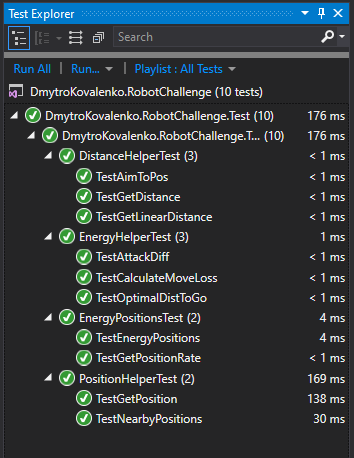
\includegraphics[scale=1]{1}
		\caption{Результат виконання тестів}
	\end{figure}
	
	\section*{Висновок}
	Під час виконання лабораторної роботи, я реалізував власний алгоритм руху роботів, з допомогою якого вони зможуть рухатися, колекціонувати енергію та створювати нових, а також розробив Unit-тести для перевірки роботи цього алгоритму.
	
	 
\end{normalsize}
\end{document}
